\documentclass[a4paper,twoside]{article}

\usepackage{apalike}
\usepackage{SCITEPRESS}
\usepackage{amssymb}
\usepackage{amstext}
\usepackage{amsmath}
\usepackage{amsthm}
\usepackage{graphicx}
\usepackage{multicol}
\usepackage[small]{caption}
\usepackage{subfloat}

\usepackage{tikz}



\begin{document}


%%%%%%%%%%%%%%%%%%%%%%%%%%%%%%%%%%%%%%%%%%%%%%%%%%%%%%%%%%%%%%%%%%%%%%%%%%%%%%%%
%%%                               80 COLONNES                                %%%
%%%%%%%%%%%%%%%%%%%%%%%%%%%%%%%%%%%%%%%%%%%%%%%%%%%%%%%%%%%%%%%%%%%%%%%%%%%%%%%%


\title{Lessons Learned through Actual Implementation of MAC/RDC Protocols
       on 802.15.4 Radio Medium: the Case of S-CoSenS}


\author{
\authorname{K\'evin Roussel, Ye-Qiong Song and Olivier Zendra}
\affiliation{LORIA/INRIA Nancy Grand-Est,\\
             Universit\'e de Lorraine,\\
             615, rue du Jardin Botanique,\\
             54600 Villers-L\`es-Nancy, France}
\email{\texttt{\{Kevin.Roussel,Ye-Qiong.Song,Olivier.Zendra\}@inria.fr}}
}


\keywords{Wireless Sensor Networks, Internet of Things, Heavy Load, QoS,
          MAC/RDC protocols, S-CoSenS, ContikiMAC}


%Nécessité de s'intéresser au cas où les réseaux de WSN ont de fortes charges
%à transmettre, ne serait-ce que ponctuellement ("bursts").

%Std 802.15.4 : délai entre réception d'un paquet et envoi d'un acquittement
%entre deux paquets successifs => rarement respectés.


\abstract{Implementing new, high-performance MAC/RDC protocols requires
real-time features, to be able to synchronize correctly between different
unrelated devices. Such features are highly desirable for operating wireless
sensor networks (WSN) that are designed to be part of the Internet of Things
(IoT). Unfortunately the operating systems commonly used in this domain
cannot provide such features.\\
In this article, we describe our implementation of a high-performance MAC/RDC
protocol, S-CoSenS, on RIOT OS, a real-time operating system for wireless
sensor networks (WSN) and the Internet of Things (IoT).\\
We then evaluate the performances of our implementation, by comparing it with
the well-known ContikiMAC protocol (running on Contiki OS), through
simulations running on the Cooja emulator. We focus on QoS results,
especially under heavy network loads.\\
Our results show that our protocol performs very well, bringing noticeable
improvements over ContikiMAC results under a large spectrum of network loads
and configurations.}


\onecolumn \maketitle \normalsize \vfill

%%%%%%%%%%%%%%%%%%%%%%%%%%%%%%%%%%%%%%%%%%%%%%%%%%%%%%%%%%%%%%%%%%%%%%%%%%%%%

\section{\uppercase{Introduction}}

TODO.


%%%%%%%%%%%%%%%%%%%%%%%%%%%%%%%%%%%%%%%%%%%%%%%%%%%%%%%%%%%%%%%%%%%%%%%%%%%%%

\section{\uppercase{WSN Software platforms}}

Specialized OSes for the resource-constrained devices that constitute
wireless sensor networks have been designed, published, and made available
for quite a long time.


The current reference OS in the domain of WSN and IoT is \emph{Contiki}
\cite{ContikiOS}. It is an open-source OS, which was first released
in 2002. It is also at the origin of many assets: we can mention, among
many others, the low-power Rime network stack \cite{Rime}, or the Cooja
advanced network simulator \cite{Cooja}.

Contiki is very lightweight and well adapted to motes and
resource-constrained devices. It is coded in standard C language, which
makes it relatively easy to learn and program. It offers an event-based
kernel, implemented using cooperative multithreading, and a complete
network stack. All of these features and advantages have made
Contiki widespread, making it the reference OS when it comes to WSN.

Contiki developers also have made advances in the MAC/RDC domain: many
of them have been implemented as part of the Contiki network stack, and
a specifically developed, ContikiMAC, has been published in 2011
\cite{ContikiMAC} and implemented into Contiki as the default
RDC protocol (designed to be used with standard CSMA/CA as MAC layer).

Consequently, we naturally decided, as a comparison reference our first tests,
to use the Contiki software platform: the ContikiOS, the ContikiMAC RDC
protocol, the standard CSMA/CA MAC layer, and the Rime network layer, used
on the IEEE 802.15.4 physical wireless/radio protocol.

\bigskip

However, Contiki's extremely compact footprint and high optimization comes
at the cost of some limitations that prevented us from using it as our
software platform.

Contiki OS is indeed not a real-time OS: the processing of ``events''---using
Contiki's terminology---is made by using the kernel's scheduler, which is
based on cooperative multitasking (using ``protothreads''; this also implies
restrictions on the use of the \texttt{switch} construct of the C language).
This scheduler only triggers at a specific, pre-determined rate; on
the platforms we're interested in, this rate is fixed to 128~Hz:
this corresponds to a time skew of up to 8~milliseconds
(8000~microseconds) to process an event, interruption management being
one of the possible events. Such a large granularity is clearly
a huge problem when implementing high-performance MAC/RDC protocols,
where a time granularity of 320~microseconds is needed, corresponding
to one backoff period (BP). The only ``real-time-oriented'' feature
of the system, \texttt{rtimer} does not solve these problems, because
of its deep limitations:
\begin{itemize}
\item only one instance is available;
\item it is impossible to call most Contiki functions---like those from
the kernel or the network stack---from the \texttt{rtimer} callbacks,
trying to do so provoking crashes or unexpected behavior.
\end{itemize}

For all these reasons, we were unable to use Contiki OS to develop and
implement our high-performance MAC/RDC protocols. We definitely needed
an OS with efficient real-time features and event handling mechanism.

\bigskip

Consequently, we focused our interest on \emph{RIOT OS} \cite{RIOT}.

This new system---first released in 2013---is also open-source and
specialized in the domain of low-power, embedded wireless sensors.
It offers many useful features, that we will now describe.

It provides the basic benefits of an OS: portability (it has been ported
to many devices powered by ARM, MSP430, and---more recently---AVR
microcontrollers) and a comprehensive set of features, including
a network stack.

Moreover, it offers key features that are otherwise yet unknown in
the WSN/IoT domain, the most important for us being:
\begin{itemize}
\item an efficient, interrupt-driven, tickless micro-kernel providing
      pre-emptive multitasking;
\item a highly efficient use of \emph{hardware timers}: all of them can be
      used concurrently (especially since the kernel is tickless), offering
      the ability to schedule actions with high precision; on low-end
      devices, based on MSP430 architecture, events can be scheduled
      with a resolution of 30~microseconds, instead of 8000~microseconds
      for Contiki OS.
\end{itemize}
These features are what make RIOT a full-fledged \emph{real-time} operating
system.

Thus, RIOT is a powerful real-time operating system, adapted to the
limitations of deeply embedded hardware microcontrollers, while offering
state-of-the-art techniques (preemptive multitasking, tickless scheduler,
optimal use of hardware timers) that---we believe---makes it one of
the most suitable OSes of the embedded and real-time world.


%%%%%%%%%%%%%%%%%%%%%%%%%%%%%%%%%%%%%%%%%%%%%%%%%%%%%%%%%%%%%%%%%%%%%%%%%%%%%

\section{\uppercase{Protocols}}
\label{SectProtoDescription}

\subsection{The ContikiMAC RDC protocol}

It is currently the default RDC protocol proposed by the Contiki OS.
This protocol is designed to work under the classical CSMA/CA MAC layer,
and is based on the \emph{Low-Power Listening} (LPL) paradigm.

It is technically a derivative of the classical X-MAC protocol \cite{XMAC}:
its basic principle, fundamentally asynchronous, is that every node keeps
its radio transceiver off as much as possible, only waking it up for short
delay of radio medium listening at a fixed rate (by default, eight times
per second in ContikiMAC). If, during the short amount of time the radio
transceiver is on, data is sensed on the medium, the radio transceiver
is kept on until the whole transmission is done; otherwise, the node
goes back into ``radio silence mode'' to save energy.
This ability to automatically adapt the duration of transceiver activity
to the live traffic on radio channel is what makes ContikiMAC a
\emph{traffic auto-adaptative} (or \emph{self-adaptative}) protocol,
at least up to a certain extent.

When a node has to emit a packet, it continuously emits it until the
intended receiver nodes ``wakes up'' its radio transceiver, receives
the transmitted data, and sends back an acknowledgement.

The first specificity of ContikiMAC is that, during transmission, instead
of emitting a specific preamble until the receiver is ready, then sending
it the actual data packet, the data packet is directly emitted by the
sender---it is its own preamble---so that receiver(s) can directly receive
and acknowledge the data packet as soon as its radio is ready (see figure
\ref{FigContikiMACDutyCycle} hereafter).

\begin{figure}[!h]
\centering
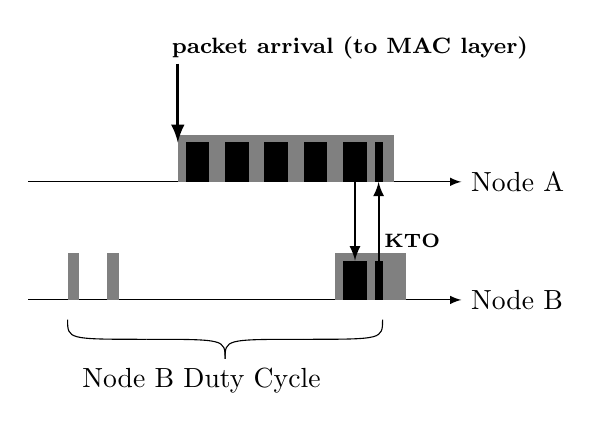
\begin{tikzpicture}[>=latex]
%sender
\draw[->] (0,  1cm) -- +(5.5cm, 0);
\draw[anchor=west] (5.5cm, 1cm) node {Node A};
\fill[gray] (1.9cm, 1cm) rectangle +(2.75cm, 0.6cm);
%packet ready to send
\draw[->,very thick] (1.9cm, 2.5cm) -- +(0, -1cm);
\draw[anchor=west] (1.7cm, 2.7cm)
     node {\footnotesize \textbf{packet arrival (to MAC layer)}};
%receiver
\draw[->] (0, -0.5cm) -- +(5.5cm, 0);
\draw[anchor=west] (5.5cm, -0.5cm) node {Node B};
%wakeup times
\fill[gray] (0.5cm, -0.5cm) rectangle +(0.15cm, 0.6cm);
\fill[gray] (1cm, -0.5cm) rectangle +(0.15cm, 0.6cm);
\fill[gray] (3.9cm, -0.5cm) rectangle +(0.9cm, 0.6cm);
\draw[anchor=west] (4.4cm, 0.25cm) node {\scriptsize \textbf{KTO}};
%packet sent
\foreach \x in {1,2,3,4,5}
{
  \fill[black] (1.5cm + \x * 0.5cm, 1cm) rectangle +(0.3cm, 0.5cm);
}
%packet received
\fill[black] (4cm, -0.5cm) rectangle +(0.3cm, 0.5cm);
\draw[->,thick] (4.15cm, 1cm) -- +(0, -1cm);
%ACK
\fill[black] (4.4cm, -0.5cm) rectangle +(0.1cm, 0.5cm);
\draw[->,thick] (4.45cm, 0cm) -- +(0, 1cm);
\fill[black] (4.4cm, 1cm) rectangle +(0.1cm, 0.5cm);
%brace
\draw (0.5cm, -0.75cm) .. controls +(0, -0.25cm) .. +(1cm, -0.25cm);
\draw (1.5cm, -1cm)    .. controls +(1cm, 0)     .. +(1cm, -0.25cm);
\draw (2.5cm, -1.25cm) .. controls +(0, 0.25cm)  .. +(1cm, 0.25cm);
\draw (3.5cm, -1cm)    .. controls +(1cm, 0)     .. +(1cm, 0.25cm);
%brace legend
\draw[anchor=north] (2.2cm,-1.25cm) node {Node B Duty Cycle};
\end{tikzpicture}
\caption{Transmission of a data packet with the ContikiMAC protocol.\\
         Gray boxes represent radio transceiver activation, while
         black boxes represent packets' transmissions.}
\label{FigContikiMACDutyCycle}
\end{figure}

The second specificity is the presence of an optimization mechanism named
\emph{``transmission phase lock''}: senders note the time when they receive
acknowledgement from receivers, and according to the known rate of radio
wake-up, deduce the subsequent expected times when these receivers are
supposed to be ready to receive packets. Thus, senders can synchronize
with nodes that have previously received their transmissions, and can
send their next packets at the optimal period to minimize the useless
transmission of packets when the intended receiver is offline. The
result of this mechanism is shown in figure \ref{FigContikiMACPhaseLock}
hereafter.

\begin{figure}[!h]
\centering
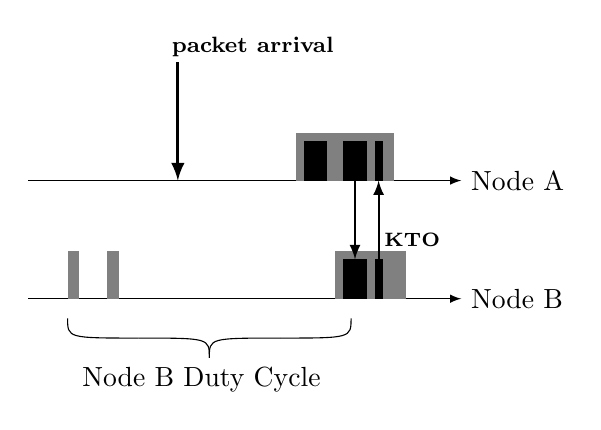
\begin{tikzpicture}[>=latex]
%sender
\draw[->] (0,  1cm) -- +(5.5cm, 0);
\draw[anchor=west] (5.5cm, 1cm) node {Node A};
\fill[gray] (3.4cm, 1cm) rectangle +(1.25cm, 0.6cm);
%packet ready to send
\draw[->,very thick] (1.9cm, 2.5cm) -- +(0, -1.5cm);
\draw[anchor=west] (1.7cm, 2.7cm)
     node {\footnotesize \textbf{packet arrival}};
%receiver
\draw[->] (0, -0.5cm) -- +(5.5cm, 0);
\draw[anchor=west] (5.5cm, -0.5cm) node {Node B};
%wakeup times
\fill[gray] (0.5cm, -0.5cm) rectangle +(0.15cm, 0.6cm);
\fill[gray] (1cm, -0.5cm) rectangle +(0.15cm, 0.6cm);
\fill[gray] (3.9cm, -0.5cm) rectangle +(0.9cm, 0.6cm);
\draw[anchor=west] (4.4cm, 0.25cm) node {\scriptsize \textbf{KTO}};
%packet sent
\foreach \x in {4,5}
{
  \fill[black] (1.5cm + \x * 0.5cm, 1cm) rectangle +(0.3cm, 0.5cm);
}
%packet received
\fill[black] (4cm, -0.5cm) rectangle +(0.3cm, 0.5cm);
\draw[->,thick] (4.15cm, 1cm) -- +(0, -1cm);
%ACK
\fill[black] (4.4cm, -0.5cm) rectangle +(0.1cm, 0.5cm);
\draw[->,thick] (4.45cm, 0cm) -- +(0, 1cm);
\fill[black] (4.4cm, 1cm) rectangle +(0.1cm, 0.5cm);
%brace
\draw (0.5cm, -0.75cm) .. controls +(0, -0.25cm) .. +(0.9cm, -0.25cm);
\draw (1.4cm, -1cm)    .. controls +(0.9cm, 0)   .. +(0.9cm, -0.25cm);
\draw (2.3cm, -1.25cm) .. controls +(0, 0.25cm)  .. +(0.9cm, 0.25cm);
\draw (3.2cm, -1cm)    .. controls +(0.9cm, 0)   .. +(0.9cm, 0.25cm);
%brace legend
\draw[anchor=north] (2.2cm,-1.25cm) node {Node B Duty Cycle};
\end{tikzpicture}
\caption{``Transmission Phase Lock'': After the transmission in figure
\ref{FigContikiMACDutyCycle} occured, node A knows when to send packets
so that node B is ready to receive them, even though both nodes have
different duty cycle phases.}
\label{FigContikiMACPhaseLock}
\end{figure}

The third feature specific to ContikiMAC is the ability to send in
a single \emph{burst} a whole lot of queued packets when those are all
destined to a same receiver. This is implemented thanks to a keep-in-wakeup
timeout period (KTO) observed by ContikiMAC after each packet reception
(as shown in figures \ref{FigContikiMACDutyCycle} and
\ref{FigContikiMACPhaseLock}).


%%%%%%%%%%%%%%%%%%%%%%%%%%%%%%%%%%%%%%%%%%%%%%%%%%%%%%%%%%%%%%%%%%%%%%%%%%%%%

\subsection{Our first design: the S-CoSenS RDC protocol}

The first RDC protocol we wanted to implement is S-CoSenS, which
is designed to work on top of the IEEE 802.15.4 physical layer. Like
ContikiMAC, it is designed to work with the classical (i.e.: beacon-less)
CSMA/CA MAC layer.

It is an evolution of the already published CoSenS protocol \cite{CosensConf}:
it adds to the latter a sleeping period for energy saving.
Thus, the basic principle of S-CoSenS is to delay the forwarding (routing)
of received packets, by dividing the radio duty cycle in three periods:
a sleeping period (SP), a waiting period (WP) where the radio medium
is listened by routers for collecting incoming 802.15.4 packets, and
finally a burst transmission period (TP) for emitting adequately
the packets enqueued during WP.

The main advantage of S-CoSenS is its ability to adapt dynamically to the
wireless network throughput at runtime, by calculating for each radio duty
cycle the length of SP and WP, according to the number of relayed
packets during previous cycles. Note that the set of the SP and the WP
of a same cycle is named \emph{subframe}; it is the part of a S-CoSenS
cycle whose length is computed and known \textit{a priori}; on the contrary,
TP duration is always unknown up to its very beginning, because it depends
on the amount of data successfully received during the WP that precedes it.

Moreover, the computation of WP duration follows a ``sliding average''
algorithm, where WP average for each duty cycle is computed as:
\begin{eqnarray*}
&&
\overline{\mathrm{WP}_{n}} = \alpha \cdot \overline{\mathrm{WP}_{n-1}}
                + (1 - \alpha) \cdot \mathrm{WP}_{n-1}
\\ &&
\mathrm{WP}_{n} = \max ( \mathrm{WP}_{min},
                  \min ( \overline{\mathrm{WP}_{n}}, \mathrm{WP}_{max} ) )
\end{eqnarray*}
where $\overline{\mathrm{WP}_{n}}$ and $\overline{\mathrm{WP}_{n-1}}$
are respectively the average WP length at $n^{\mathrm{th}}$ and
$(n-1)^{\mathrm{th}}$ cycle, while $\mathrm{WP}_{n}$ and $\mathrm{WP}_{n-1}$
are the actual length of respectively the $n^{\mathrm{th}}$ and
$(n-1)^{\mathrm{th}}$ cycles; $\alpha$ is a parameter between 0 and 1
representing the relative weight of the history in the computation,
and $\mathrm{WP}_{min}$ and $\mathrm{WP}_{max}$ are high and low limits
imposed by the programmer to the WP duration.

The local synchronization between a S-CoSenS router and the leaf nodes
that take it as parent is done thanks to a beacon packet, that is broadcasted
by the router at the beginning of each duty cycle. This beacon contains the
duration (in microseconds) of the SP and WP for the currently beginning
duty cycle.

The whole S-CoSenS duty cycle workflow for a router is summarized in figure
\ref{FigSCosensDutyCycle} hereafter.

\begin{figure}[!h]
\centering
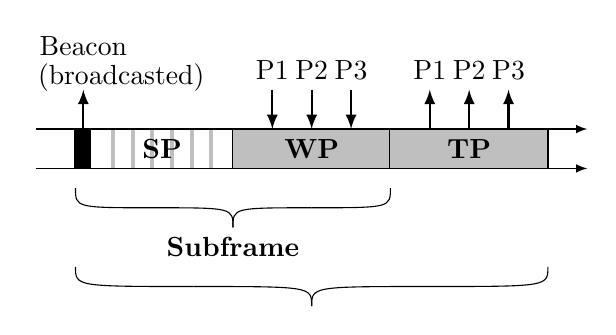
\begin{tikzpicture}[>=latex]
%beacon
\fill[black] (0cm, -0.25cm) rectangle +(0.2cm, 0.5cm);
\draw[->,thick] (0.1cm, 0.25cm) -- +(0, 0.5cm);
\draw (0.1cm, 1.3cm) node {Beacon};
\draw[anchor=west] (-0.6cm, 0.9cm) node {(broadcasted)};
%SP
\draw[thick] (0cm, -0.25cm) -- +(0, 0.5cm);
%regular wake-ups during SP
\foreach \x in {1,2,3,4,5,6}
{
  \fill[lightgray] (0.2cm + \x * 0.25cm, -0.25cm) rectangle +(0.05cm, 0.5cm);
}
\draw (1.1cm, 0) node {\textbf{SP}};
%WP
\draw[thick] (2cm, -0.25cm) -- +(0, 0.5cm);
\fill[lightgray] (2cm, -0.25cm) rectangle +(2cm, 0.5cm);
\draw (3cm, 0) node {\textbf{WP}};
%TP
\draw[thick] (4cm, -0.25cm) -- +(0, 0.5cm);
\fill[lightgray] (4cm, -0.25cm) rectangle +(2cm, 0.5cm);
\draw (5cm, 0) node {\textbf{TP}};
\draw[thick] (6cm, -0.25cm) -- +(0, 0.5cm);
%time axes
\draw[->] (-0.5cm,  0.25cm) -- +(7cm, 0);
\draw[->] (-0.5cm, -0.25cm) -- +(7cm, 0);
%RX packets
\draw[->,thick] (2.5cm, 0.75cm) -- +(0, -0.5cm);
\draw (2.5cm, 1cm) node {P1};
\draw[->,thick] (3cm, 0.75cm) -- +(0, -0.5cm);
\draw (3cm, 1cm) node {P2};
\draw[->,thick] (3.5cm, 0.75cm) -- +(0, -0.5cm);
\draw (3.5cm, 1cm) node {P3};
%TX packets
\draw[->,thick] (4.5cm, 0.25cm) -- +(0, 0.5cm);
\draw (4.5cm, 1cm) node {P1};
\draw[->,thick] (5cm, 0.25cm) -- +(0, 0.5cm);
\draw (5cm, 1cm) node {P2};
\draw[->,thick] (5.5cm, 0.25cm) -- +(0, 0.5cm);
\draw (5.5cm, 1cm) node {P3};
%first brace: subframe
\draw (0cm, -0.5cm)  .. controls +(0, -0.25cm) .. +(1cm, -0.25cm);
\draw (1cm, -0.75cm) .. controls +(1cm, 0)     .. +(1cm, -0.25cm);
\draw (2cm, -1cm)    .. controls +(0, 0.25cm)  .. +(1cm, 0.25cm);
\draw (3cm, -0.75cm) .. controls +(1cm, 0)     .. +(1cm, 0.25cm);
\draw (2cm, -1.25cm) node {\textbf{Subframe}};
%second brace: whole cycle
\draw (0cm, -1.5cm)    .. controls +(0, -0.25cm) .. +(1.5cm, -0.25cm);
\draw (1.5cm, -1.75cm) .. controls +(1.5cm, 0)   .. +(1.5cm, -0.25cm);
\draw (3cm, -2cm)      .. controls +(0, 0.25cm)  .. +(1.5cm, 0.25cm);
\draw (4.5cm, -1.75cm) .. controls +(1.5cm, 0)   .. +(1.5cm, 0.25cm);
\end{tikzpicture}
\caption{A typical S-CoSenS router cycle.\\
         The gray strips in the SP represents the short wake-up-and-listen
         periods used for inter-router communication.}
\label{FigSCosensDutyCycle}
\end{figure}

Note that in contrast to ContikiMAC, S-CoSenS is based on the \emph{Receiver
Initiated} (RI) paradigm, whose the classical RI-MAC protocol \cite{RIMAC}
is one of the better known application.
Local synchronization between a S-CoSenS router and its leaf nodes, done
as seen hereabove with the regular emission of a beacon, relies on the
\emph{Low-Power Probing} (LPP) paradigm.
On the other hand, synchronization and communication between different
S-CoSenS routers, made thanks to short regular wake-up-and-listen periods,
is based on the Low-Power Listening (LPL) paradigm (like the ContikiMAC
protocol to which this mechanism is very similar, see on figure
\ref{FigSCosensDutyCycle}).

An interesting property of S-CoSenS is that leaf (i.e.: non-router) nodes
always have their radio transceiver offline, except when they have packets
to send. When a data packet is generated on a leaf node, the latter wakes up
its radio transceiver, listens and waits to the first beacon emitted by
an S-CoSenS router, then sends its packet using CSMA/CA at the beginning
of the WP described in the beacon it received. A leaf node will put its
transceiver offline during the delay between the beacon and that WP
(that is: the SP of the router that emitted the received beacon), and
will go back to sleep mode once its packet is transmitted.
All of this procedure is shown in figure \ref{FigSCoSenSPktTx}.

\begin{figure}[!h]
\centering
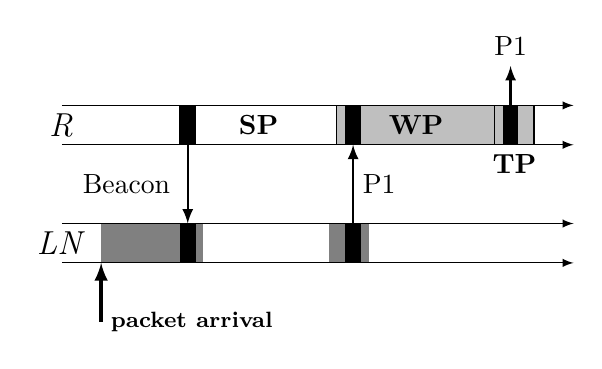
\begin{tikzpicture}[>=latex]
%%router
\draw (-0.5cm, 0) node {\large \textit{R}};
%sp
\draw[thick] (1cm, -0.25cm) -- +(0, 0.5cm);
\draw (2cm, 0) node {\textbf{SP}};
%wp
\draw[thick] (3cm, -0.25cm) -- +(0, 0.5cm);
\fill[lightgray] (3cm, -0.25cm) rectangle +(2cm, 0.5cm);
\draw (4cm, 0) node {\textbf{WP}};
%tp
\draw[thick] (5cm, -0.25cm) -- +(0, 0.5cm);
\fill[lightgray] (5cm, -0.25cm) rectangle +(0.5cm, 0.5cm);
\draw (5.25cm, -0.5cm) node {\textbf{TP}};
\draw[thick] (5.5cm, -0.25cm) -- +(0, 0.5cm);
%time axes
\draw[->] (-0.5cm,  0.25cm) -- +(6.5cm, 0);
\draw[->] (-0.5cm, -0.25cm) -- +(6.5cm, 0);
%%leaf node
\draw (-0.5cm, -1.5cm) node {\large \textit{LN}};
%radio activity
\fill[gray] (0cm, -1.25cm) rectangle +(1.3cm, -0.5cm);
\fill[gray] (2.9cm, -1.25cm) rectangle +(0.5cm, -0.5cm);
%beacon
\fill[black] (1cm, -0.25cm) rectangle +(0.2cm, 0.5cm);
\draw[->,thick] (1.1cm, 0.25cm) -- +(0, -1.5cm);
\draw[anchor=east] (1cm, -0.75cm) node {Beacon};
\fill[black] (1cm, -1.25cm) rectangle +(0.2cm, -0.5cm);
%packet generation
\draw[->,very thick] (0cm, -2.5cm) -- +(0, 0.75cm);
\draw[anchor=west] (0cm, -2.5cm)
     node {\footnotesize \textbf{packet arrival}};
%TX leaf->router
\fill[black] (3.1cm, -1.25cm) rectangle +(0.2cm, -0.5cm);
\draw[->,thick] (3.2cm, -1.25cm) -- +(0, 1cm);
\draw[anchor=west] (3.2cm, -0.75cm) node {P1};
\fill[black] (3.1cm, -0.25cm) rectangle +(0.2cm, 0.5cm);
%TX router->...
\fill[black] (5.1cm, -0.25cm) rectangle +(0.2cm, 0.5cm);
\draw[->,thick] (5.2cm, 0.25cm) -- +(0, 0.5cm);
\draw (5.2cm, 1cm) node {P1};
%time axes
\draw[->] (-0.5cm, -1.25cm) -- +(6.5cm, 0);
\draw[->] (-0.5cm, -1.75cm) -- +(6.5cm, 0);
\end{tikzpicture}
\caption{A typical transmission of a data packet with the S-CoSenS protocol
         between a leaf node and a router.}
\label{FigSCoSenSPktTx}
\end{figure}

We thus need to synchronize with enough accuracy different devices (that
can be based on different hardware platforms) on duty cycles whose periods
are dynamically calculated at runtime, with resolution that needs to be
in the sub-millisecond range. This is where RIOT OS advanced real-time
features really shine, while the other comparable OSes are
for that purpose definitely lacking.

\bigskip

We have implemented S-CoSenS under RIOT OS, and evaluated it by comparing
to the ContikiMAC + CSMA/CA couple under Contiki OS.

As there was no standard implementation in RIOT OS network stack of
the CSMA/CA described in the 802.15.4 protocol, our implementation of
S-CoSenS currently also includes that MAC layer. This shall be changed
in future production-ready implementations.


%%%%%%%%%%%%%%%%%%%%%%%%%%%%%%%%%%%%%%%%%%%%%%%%%%%%%%%%%%%%%%%%%%%%%%%%%%%%%

\section{\uppercase{Method and Benchmark}}

For our first experiments, we used, for practical reasons, the Cooja
simulator rather than actual hardware. All the simulated nodes are
virtual Zolertia Z1 motes, well-known industrial MSP430-based devices.

We have implemented test applications under both Contiki and RIOT OS, and
made first tests by performing simulations of a basic 802.15.4 PAN
(Personal Area Network) constituted of a ``router'', and ten motes
acting as ``leaf nodes''. The ten nodes regularly send data packets to
the router, that retransmits these data packets to a nearby ``sink'' device.
Both the router and the ten nodes use exclusively the S-CoSenS RDC/MAC
protocol. This is summarized in figure \ref{FigPANtest}.

\begin{figure}[!h]
\centering
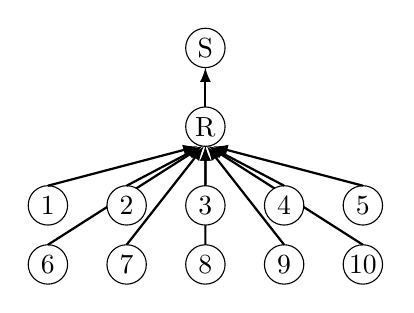
\begin{tikzpicture}[>=latex]
%sink
\draw (0, 1cm) circle (0.25cm); \draw (0, 1cm) node {S};
%router to sink link
\draw[->,thick] (0, 0.25cm) -- (0, 0.75cm);
%router
\draw (0, 0) circle (0.25cm); \draw (0, 0) node {R};
%leaf nodes (lower)
\foreach \x in {6,7,8,9,10}
{
  \fill[white] (\x * 1cm - 8cm, -1.75cm) circle (0.25cm);
  \draw (\x * 1cm - 8cm, -1.75cm) circle (0.25cm);
  \draw (\x * 1cm - 8cm, -1.75cm) node {\x};
  % link to router
  \draw[->,thick] (\x * 1cm - 8cm, -1.5cm)
                  -- (\x * 0.02cm - 0.16cm, -0.25cm);
}
%leaf nodes (upper)
\foreach \x in {1,2,3,4,5}
{
  \fill[white] (\x * 1cm - 3cm, -1cm) circle (0.25cm);
  \draw (\x * 1cm - 3cm, -1cm) circle (0.25cm);
  \draw (\x * 1cm - 3cm, -1cm) node {\x};
  % link to router
  \draw[->,thick] (\x * 1cm - 3cm, -0.75cm)
                  -- (\x * 0.05cm - 0.15cm, -0.25cm);
}
\end{tikzpicture}
\caption{Functional schema of our virtual test PAN.}
\label{FigPANtest}
\end{figure}

We then performed simulations on this virtual PAN, varying several parameters
of the ContikiMAC RDC protocol, under moderately-heavy to extreme network
loads. The loads were generated by the application loaded on the 10 leaf
nodes: they were programmed to generate large 802.15.4 network packets
(90 bytes of payload, which translates to an actual packet size of
111 bytes) at a fixed rate, with random jitters in the interval of
$[ 0.5 L , 1.5  L ]$, with $L$ being the targeted inter-arrival
period. The different setups are described in table \ref{TblDataRates}:
the table gives the average inter-arrival period between two consecutive
packets sent by each mote, the average number of packets emitted every
second for the 10 leaf nodes, and the expected resulting data rate.

\begin{table}[htb]
\centering
\begin{tabular}{|l|p{1.25cm}|r|r|}
\hline
Setup     &  Inter-Arrival  & Pkts/s & Data Rate \\
\hline
Moderate  & 1500 ms &   6.7  &  5,867 bit/s \\ 
High      & 1000 ms &  10    &  8,800 bit/s \\
Very High &  500 ms &  20    & 17,600 bit/s \\
Extreme   &  100 ms & 100    & 88,000 bit/s \\
\hline
\end{tabular}
\caption{Transmission data rates used on leaf nodes.}
\label{TblDataRates}
\end{table}

For each scenario, we performed two kinds of simulations:
\begin{itemize}
\item a \emph{fixed packet number simulation}, during which each node emits
500 packets at the fixed rate, then turns off; the simulation ends when all
nodes have transmitted their quota of packets;

\item a \emph{fixed duration simulation}, during which each node emits an
unspecified number of packets at the fixed rate; the simulation ends after
10 minutes.
\end{itemize}

These different kinds of simulations allow us to easily compute respectively
packet reception rate (PRR) and duty cycle statistics, as we will now see
in the next section.


%%%%%%%%%%%%%%%%%%%%%%%%%%%%%%%%%%%%%%%%%%%%%%%%%%%%%%%%%%%%%%%%%%%%%%%%%%%%%

\section{\uppercase{Results and Discussion}}

\subsection{Quality of Service (QoS)}

We quantify the QoS, in our simulations of WSN, by the number of packets
that arrive to their destination, that is: the number of packets that are
sent from one of the leaf nodes, relayed by the router, and are actually
received by the sink.

Using the \emph{fixed packet number simulations}, we can easily compute the
rate of packets that arrive to destination, compared to the known number
of packets emitted by the nodes.

Thus, we were able to determine that the only parameter that has actually
influence on the QoS is the length of the duty cycle on S-CoSenS, which
corresponds in the ContikiMAC RDC protocol to the rate at which the radio
medium is sensed (this parameter is named
\texttt{NETSTACK\_CONF\_RDC\_CHANNEL\_CHECK\_RATE} in Contiki source code).
Its default value is 8, meaning the radio channel is checked eight times
per second; this parameter is actually given in Hertz.
In S-CoSenS, the default duration for the subframe is 100 ms.

Note that we also allowed, on Contiki, the the standard CSMA/CA MAC layer
to perform up to seven retries for a given data packet, by setting the
\texttt{CSMA\_CONF\_MAX\_MAC\_TRANSMISSIONS}
parameter to 8 in Contiki source code. This was done in order to put it
on par with S-CoSenS default configuration, where a packet can by default
be transmitted up to 8 times before being cancelled.
Attention: the ``retry'' term does not have the same signification
under S-CoSenS---where it specifies the reemission of \emph{one} instance of
a packet---than on ContikiMAC where it specifies a new duty cycle during
which the packet is reemitted an unspecified number of times. This is
the consequence of the fundamental difference in design between the two
protocols (see section \ref{SectProtoDescription} above).

This default value of 8~Hz/125~ms only gives very poor results for ContikiMAC.
To obtain fairer results for the latter protocol, we changed that parameter's
value, and doubled it up to 64~Hz/16~ms.

The results we obtained are shown in figures \ref{FigSuccessRate8Hz} to
\ref{FigSuccessRateSCoSenS}. These figures show the rates of packets
successfully arrived to their destination, according to the duty cycle
duration (with ContikiMAC: via changing the channel check rate parameter).
These results are obtained with fixed packet number simulations.

\begin{figure}
  \centering
  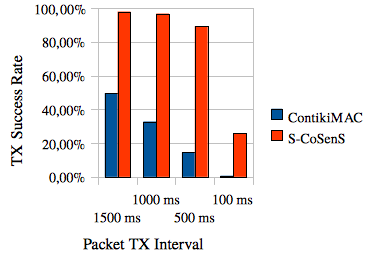
\includegraphics[width=7.5cm]{graphes/QoS8Hz.png}
  \caption{QoS results for 125~ms duty cycle}
  \label{FigSuccessRate8Hz}
\end{figure}
\begin{figure}
  \centering
  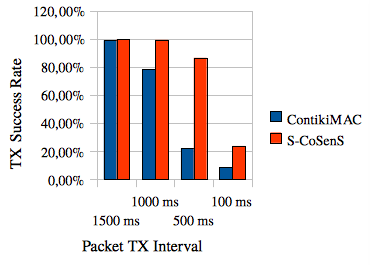
\includegraphics[width=7.5cm]{graphes/QoS16Hz.png}
  \caption{QoS results for 62~ms duty cycle}
  \label{FigSuccessRate16Hz}
\end{figure}
\begin{figure}
  \centering
  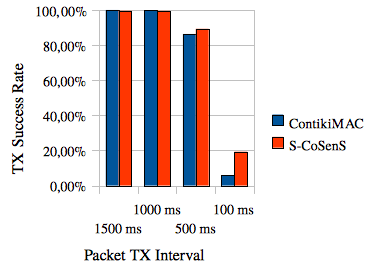
\includegraphics[width=7.5cm]{graphes/QoS32Hz.png}
  \caption{QoS results for 31~ms duty cycle}
  \label{FigSuccessRate32Hz}
\end{figure}
\begin{figure}
  \centering
  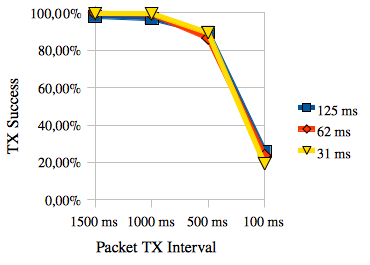
\includegraphics[width=7.5cm]{graphes/QoSstabilitySCoSenS.png}
  \caption{Combined QoS results for S-CoSenS,
           according to duty cycle duration}
  \label{FigSuccessRateSCoSenS}
\end{figure}

The data shown in figures \ref{FigSuccessRate8Hz} to
\ref{FigSuccessRateSCoSenS} show us many facts:

\begin{itemize}

\item ContikiMAC QoS increases with Channel Check Rate.

\item S-CoSenS QoS results are either similar or better than ContikiMAC's.

\item S-CoSenS QoS results are much more stable when the duty cycle duration
      changes than ContikiMAC's: this stability is clearly visible on figure
      \ref{FigSuccessRateSCoSenS}; thus, S-CoSenS performance is much more
      predictable, and gives most of the time the insurance of a fair
      rate of successfully transmitted packets.

\end{itemize}

Analysis of the QoS results, not visible on the figures presented here, has
also shown us that :

\begin{itemize}

\item With ContikiMAC, the packet losses are mainly due to the router.

\item With S-CoSens, the router never loses the packets it receives:
      all losses occur between leaf nodes and router.

\end{itemize}

This is not surprising, since S-CoSenS explicitly reserves a period in every
duty cycle for packet (re)transmission, while ContikiMAC doesn't provide
such a feature. We can clearly understand that under heavy network load,
a ContikiMAC router will have data to receive almost every time it wakes up
its radio transceiver; thus, it will become increasingly difficult for this
router to be able to retransmit the packet it receives with each increase
of the network traffic. That's why under such scenarii, the router node
is clearly the weak point for ContikiMAC setups, while S-CoSenS manages
to avoid these difficulties by design.


%%%%%%%%%%%%%%%%%%%%%%%%%%%%%%%%%%%%%%%%%%%%%%%%%%%%%%%%%%%%%%%%%%%%%%%%%%%%%

\subsection{End-to-end Transmission Delays}

Using the results of the same experiments, we analyzed the traces of
exchanged packets during simulations, and computed the delays that takes each
successfully transmitted packet to go from its originating leaf node up to
the sink---that is: the duration of its two-hop transmission.

The results we obtained are shown in figures \ref{FigDelays8Hz} to
\ref{FigDelaysSCoSenS}. These figures show the mean delay for
a successfully transferred packet to make its all of its two-hop trip.
Note that figures \ref{FigDelays8Hz}, \ref{FigDelays16Hz} and
\ref{FigDelays32Hz} show the delays---in their vertical axis---in
logarithmic scale, for better readability.

\begin{figure}
  \centering
  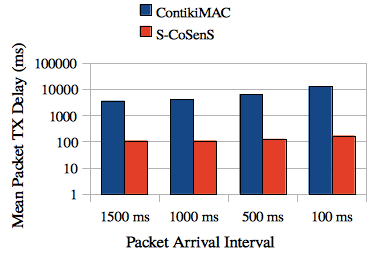
\includegraphics[width=7.5cm]{graphes/Delays8Hz.png}
  \caption{Transmission delay means for 125~ms duty cycle}
  \label{FigDelays8Hz}
\end{figure}
\begin{figure}
  \centering
  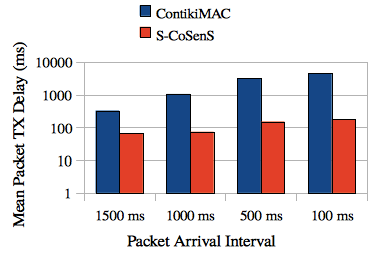
\includegraphics[width=7.5cm]{graphes/Delays16Hz.png}
  \caption{Transmission delay means for 62~ms duty cycle}
  \label{FigDelays16Hz}
\end{figure}
\begin{figure}
  \centering
  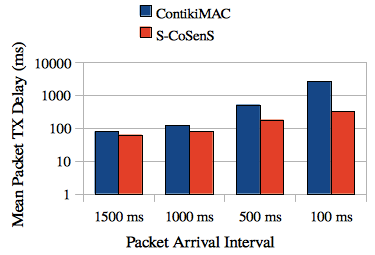
\includegraphics[width=7.5cm]{graphes/Delays32Hz.png}
  \caption{Transmission delay means for 31~ms duty cycle}
  \label{FigDelays32Hz}
\end{figure}
\begin{figure}
  \centering
  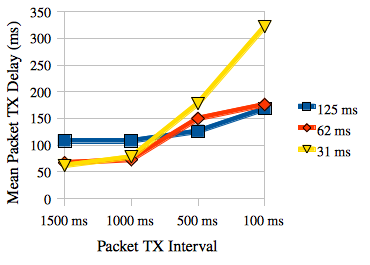
\includegraphics[width=7.5cm]{graphes/DelaysStabilitySCoSenS.png}
  \caption{Combined Transmission delay means for S-CoSenS,
           according to duty cycle duration}
  \label{FigDelaysSCoSenS}
\end{figure}

These results also indicate that:

\begin{itemize}

\item ContikiMAC delays shorten with Channel Check Rate.

\item S-CoSenS delays are always similar or shorter then than ContikiMAC's.

\item S-CoSenS delays are much more stable when the duty cycle duration
      changes. In most cases, S-CoSenS gives the insurance that packet
      transmission delays will keep under a reasonable limit.

\end{itemize}

These observation are strictly similar to those made for QoS results.

This very large increase in end-to-end transmission delays for ContikiMAC
can be interpreted as ``overzealousness'': a packet can be retransmitted
during a fixed number of retries (8 in our setups, 3 by default in Contiki);
since for ContikiMAC+CSMA/CA, an attempt to transmit a packet can be delayed
up until the radio medium is available, and consists in trying to send
a packet repetitively up to a whole duty cycle, a enormous amount of time
is elapsed before the protocol finally gives up on transmitting a given
packet.

While such an ``obstinacy'' can improve QoS by increasing transmission
success rate, it also eventually greatly increases the mean delay for
end-to-end packet transmission. In the end, one can wonder about the
interest of transmitting packets with such a great age, at the expense
of transmitting packets with more recent and meaningful data.

The configuration of the amount of retries to perform for a given
transmission is---like many other parameters---a balance between two
contradictory goals: the aim is to have a sufficient TX success rate (QoS)
while also allowing the loss and discarding of too old data. It seems
that in the scenarii we studied, S-CoSenS manages to obtain a better
trade-off between these two goals than ContikiMAC+CSMA/CA couple.


%%%%%%%%%%%%%%%%%%%%%%%%%%%%%%%%%%%%%%%%%%%%%%%%%%%%%%%%%%%%%%%%%%%%%%%%%%%%%

\subsection{Limitations and Inconsistencies}
\label{SectLimits}

The current work has of course its limitations. Its main drawback is that
\emph{it is only based on simulations.} To be truly accurate, we would need
to run these tests on actual hardware.

Moreover, we constated, during our simulations, an anomaly in the MSPSim
software (the MSP430 device simulator used by Cooja to emulate MSP430-based
motes at the cycle level \cite{MSPSim}): \emph{the delay used by the
simulator to load our large---110 bytes---IEEE 802.15.4 packets into
the CC2420 transceiver TX buffer is too long;} Table \ref{TblTXPktLoadDelays}
show the differences of delay for loading our packets between
Cooja simulations and real hardware executions.

\begin{table}
\centering
\begin{tabular}{|l|r|r|}
\hline
Setup     &  Cooja Sim.  & Hardware Test \\
\hline
RIOT OS    &   36 ticks  &  14 ticks \\ 
Contiki OS &   14 ticks  &   7 ticks \\
\hline
\end{tabular}
\caption{Delays observed for loading packets into CC2420 TX buffer.\\
Values are given in ``ticks'' of \texttt{rtimer/hwtimer}, both of these
timers incrementing at a rate of 32,768Hz. The unit is thus a fixed period
of time equal to about 30.5 microseconds.}
\label{TblTXPktLoadDelays}
\end{table}

We can see that this problem occurs whatever OS is used on the motes.
This problem seems to be caused by an overestimation of the delays caused
by the operation of the SPI bus that links the MSP430 microcontroller
to the CC2420 radio transceiver on the Z1 hardware. We didn't have time
to further investigate the problem and correct that anomaly.

We also don't know whether or not there are other inconsistencies in
the simulator software that could also alter the results of our
simulations...

Such anomalies may have an impact, and change the results obtained on real
hardware using the same scenarii and parameters. Unfortunately, we don't
have enough Z1 motes nor time to perform these real-life tests yet.

However, since the delay overestimation seems quite larger for RIOT OS
operation than for Contiki (for a reason that is still unexplained to us),
we can expect the results on real hardware to improve further for RIOT OS
than for Contiki compared to what we obtained by simulation. Consequently,
we firmly believe that the general facts we observed in our simulations
won't be overturned by these problems. That's why we still present
them in the current article.


%%%%%%%%%%%%%%%%%%%%%%%%%%%%%%%%%%%%%%%%%%%%%%%%%%%%%%%%%%%%%%%%%%%%%%%%%%%%%

\section{\uppercase{Conclusion and Future Works}}

We have build simulation scenarios to test whether our MAC/RDC protocol,
S-CoSenS, could handle heavy network loads, trying to approach the
theoretical limit of 250~kbit/s of bandwith for the underlying
IEEE 802.15.4 radio medium.

We were able to show---with the limits and preventions discussed hereabove
in section \ref{SectLimits}---that it performs quite well under these
situations, and does it better than the reference software platform, in terms
of QoS and packet transmission delays: it can handle quite gracefully some of
the heavy loads we imposed on it during our simulations, managing to obtain
a good to excellent QoS---that is: few packets lost during transmissions.
(Under extreme loads however, it becomes impossible to obtain satisfactory
results for QoS: the radio medium becoming saturated causes the MAC/RDC
layer to stall and become ineffective.)

One must also accept that there is no way to keep the very low power
consumption feature when dealing with such heavy network loads, the
motes' radio transceivers being heavily activated and solicited to
handle that charge.

\bigskip

In the future, we would like to try other, more powerful hardware platforms
with the same scenarii, and try using different MAC and RDC layers in
the network stack of the RIOT operating system.

We hope to find (a) way(s) to get a similar or better QoS than those
we observed here, while trying to optimize duty cycle statistics
to minimize the energy consumption when running WSN, whether under
light or heavy network loads.


%%%%%%%%%%%%%%%%%%%%%%%%%%%%%%%%%%%%%%%%%%%%%%%%%%%%%%%%%%%%%%%%%%%%%%%%%%%%%


\vfill
\bibliographystyle{apalike}
{\small
\bibliography{wowmom2015}}


\end{document}
